\chapter{가환 관측량, 에너지 위상, 스핀 세차}

\lectureoverview{불확정성의 정성적 의미부터 살펴본다. 두 관측량이 동시에 확정된 값을 가질 수 있는 것은 완전한 공통 고유기저를 가질 때뿐이며, 이는 두 연산자가 서로 가환하는 것과 동치이다. 이어서 유니터리 시간발전과 Schr\"odinger 방정식을 복습하고, 교환자를 고전적인 푸아송 괄호와 비교한다. 그런 다음 에너지 기저에서 시간 의존 방정식을 풀고 자기장 속 스핀에 적용한다. 마지막 계산에서는 스핀 기댓값의 세차, 일반적인 스핀 해밀토니언의 두 에너지 준위, 그리고 횡방향 기댓값과 에너지 간격의 절반에 해당하는 에너지를 가진 광자의 차이를 다룬다.}

두 상태 스핀은 여전히 가장 단순한 양자계다. 세 상태 힐베르트 공간이 그다음으로 단순한 추상적 가능성이며, 스핀 두 개만으로도 서로 직교하는 기저 상태가 네 개 생긴다. 아직 스핀 두 개를 합성하지는 않겠지만, 그 단계는 멀지 않았고 얽힘도 함께 다루게 될 것이다. 먼저 스핀 하나의 문제를 마무리하고 불확정성과 시간발전의 개념을 더 확실히 다져야 한다.

\section{두 물리량이 동시에 확정될 수 있는 경우}

좋은 측정은 반복 가능하다. 어떤 관측량을 측정해 값 \(l\)을 얻었다면, 곧바로 다시 측정했을 때도 같은 값이 나와야 한다. 따라서 첫 번째 측정은 적어도 순간적으로 계를 해당 연산자의 고유상태에 남겨 두어야 한다.
\begin{equation}
L\ket{l}=l\ket{l}.
\end{equation}
이 조작적 진술만으로도 불확정성이 생기는 정성적 이유를 드러내기에 충분하다.

두 관측량 \(L\)과 \(M\)을 동시에 측정할 수 있다고 하자. 공동 측정 후에는 측정 결과로 보고된 두 값이 모두 확정되어 있어야 한다. 따라서 측정 후 가능한 상태는 두 연산자의 동시 고유벡터여야 한다. 여기서 사용하는 유한 차원 공간에서는 다음을 만족하는 완전한 정규직교 집합 \(\{\ket{i}\}\)을 택할 수 있다.
\begin{equation}
L\ket{i}=l_i\ket{i},
\qquad
M\ket{i}=m_i\ket{i}.
\label{eq:l5-common-eigenvectors}
\end{equation}

\begin{remark}
여기서 \emph{기저}란 완전한 정규직교 기저를 뜻한다. 선형대수에서는 서로 직교하지 않는 기저도 허용하지만, 양자 상태에는 정규직교 기저가 특히 자연스럽다. 고유값이 축퇴되어 있으면 고유공간 안에 선택의 자유가 남으므로, 그 공간 안의 고유벡터는 정규직교하도록 선택할 수 있다.
\end{remark}

\begin{theorem}
유한 차원 에르미트 관측량 두 개는 완전한 공통 고유기저를 가질 때, 그리고 그때에 한해서 동시에 측정할 수 있다. 이는 두 관측량이 가환한다는 것과 동치다.
\end{theorem}

정리의 한 방향은 식~\eqref{eq:l5-common-eigenvectors}에서 바로 알 수 있다. 연산자를 한 순서로 작용시키면
\begin{align}
ML\ket{i}
&=M\bigl(l_i\ket{i}\bigr)\\
&=l_i m_i\ket{i},
\end{align}
반대 순서로 작용시키면
\begin{align}
LM\ket{i}
&=L\bigl(m_i\ket{i}\bigr)\\
&=m_i l_i\ket{i}.
\end{align}
고유값은 보통의 수이므로 \(l_i m_i=m_i l_i\)이다. 따라서 \(ML\)와 \(LM\)는 기저의 모든 원소에 동일하게 작용하며, 그러므로 모든 상태에도 동일하게 작용한다.
\begin{equation}
[L,M]\equiv LM-ML=0.
\label{eq:l5-commuting-condition}
\end{equation}

\begin{figure}[htbp]\centering
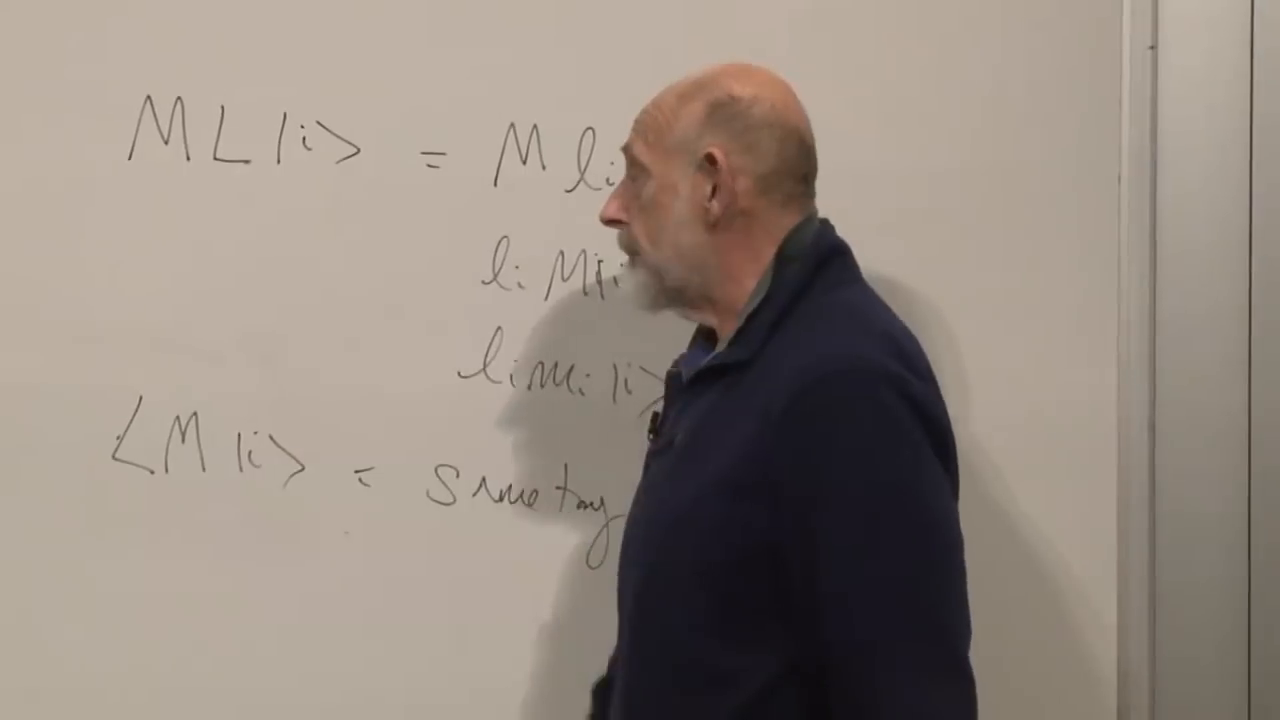
\includegraphics[width=0.86\textwidth]{lecture_05_figure_02.png}\caption{공통 고유벡터를 이용한 논증으로 \(LM-ML=[L,M]=0\)을 얻는다.}\lectureframe{00:10:30}\end{figure}

역도 성립한다. 가환하는 에르미트 연산자는 동시에 대각화할 수 있다. 한 연산자에 축퇴 고유공간이 있으면 다른 연산자는 그 고유공간을 보존하며, 그 안에서 대각화할 수 있다. 모든 고유공간에서 이 과정을 되풀이하면 완전한 공통 고유기저를 얻는다.

파울리 연산자는 처음으로 중요한 반례를 보여 준다. \(\sigma_x,\sigma_y,\sigma_z\) 중 어느 두 개도 서로 가환하지 않는다. \(\sigma_z\)의 고유상태는 위와 아래 방향이고, \(\sigma_x\)의 고유상태는 오른쪽과 왼쪽 방향이다. 한 성분을 정확히 정해 준비한 뒤 그 성분을 반복 측정할 수는 있지만, 두 성분을 동시에 정확히 정해 준비할 수는 없다. 이는 수치적 부등식을 도입하기 전부터 나타나는 불확정성이다.

나중에는 서로 가환하지 않는 관측량 두 개의 불확실성이 어떻게 서로를 제약하는지 정량화할 것이다. 여기서는 수치적 불확정성 원리를 증명하는 것이 아니다. 부등식을 다루기 전에 짚을 점은 다음과 같다. 비가환성은 상태가 두 물리량에 동시에 확정된 값을 부여하는 것을 막는다.

\begin{classroomqa}\audiencequestion{동시 측정에는 왜 공통 고유벡터가 필요한가요?}\lecturerresponse{반복 가능한 측정은 측정된 값이 확정된 상태를 남기며, 이는 측정된 연산자의 고유상태를 뜻합니다. 두 값을 함께 얻고 두 측정 모두 반복 가능하게 유지되려면, 그 결과 상태는 두 연산자의 고유상태여야 합니다. 따라서 가능한 공동 측정 결과 전체가 공통 고유기저를 이룹니다.}\end{classroomqa}

\begin{classroomqa}\audiencequestion{서로 다른 두 입자에 관한 이야기인가요?}\lecturerresponse{그럴 필요는 없습니다. \(\sigma_x\)와 \(\sigma_z\)는 이미 하나의 스핀에 작용합니다. 그러나 서로 다른 두 부분계에 작용하는 관측량은 가환합니다. \(A\otimes I\)는 \(I\otimes B\)와 가환합니다. 그래서 한 스핀의 성분과 다른 스핀의 성분을 함께 측정할 수 있습니다. 이런 계들을 합성하면 나중에 얽힘으로 이어집니다.}\end{classroomqa}

\section{유니터리 시간발전과 그 생성자}

양자역학은 상태를 정의하기까지 고전역학보다 훨씬 오랜 시간이 걸렸지만, 상태 공간을 정하고 나면 운동 법칙은 간결하다. 다음과 같이 두자.
\begin{equation}
\ket{\psi(t)}=U(t)\ket{\psi(0)}.
\label{eq:l5-propagator}
\end{equation}
시간발전은 서로 구별할 수 있는 상태를 보존해야 한다. 더 나아가 모든 내적을 보존한다. 정규직교 기저에 대해
\begin{equation}
\bra{j}U^\dagger(t)U(t)\ket{i}=\delta_{ji},
\end{equation}
따라서
\begin{equation}
U^\dagger(t)U(t)=I.
\label{eq:l5-unitarity}
\end{equation}
시간발전 연산자는 유니터리다.

경과 시간이 0일 때는 \(U(0)=I\)이다. 연속성에 따르면 작은 시간 \(\epsilon\) 동안의 시간발전은 항등 연산자에서 조금만 달라진다. \(\hbar=1\)인 단위계에서 다음과 같이 쓰자.
\begin{equation}
U(\epsilon)=I-i\epsilon H+O(\epsilon^2),
\qquad
U^\dagger(\epsilon)=I+i\epsilon H^\dagger+O(\epsilon^2).
\end{equation}
식~\eqref{eq:l5-unitarity}에 대입하면
\begin{equation}
H^\dagger=H.
\end{equation}
시간발전의 생성자는 에르미트이므로 관측량이다. 바로 해밀토니안이다.

무한소 전파 연산자를 상태에 작용시키면
\begin{equation}
\ket{\psi(\epsilon)}
=\ket{\psi(0)}-i\epsilon H\ket{\psi(0)}+O(\epsilon^2).
\end{equation}
식을 정리하면 칠판에 적힌 차분 몫을 얻는다.
\begin{equation}
\frac{\ket{\psi(\epsilon)}-\ket{\psi(0)}}{\epsilon}
=-iH\ket{\psi(0)}+O(\epsilon).
\end{equation}

\begin{figure}[htbp]\centering
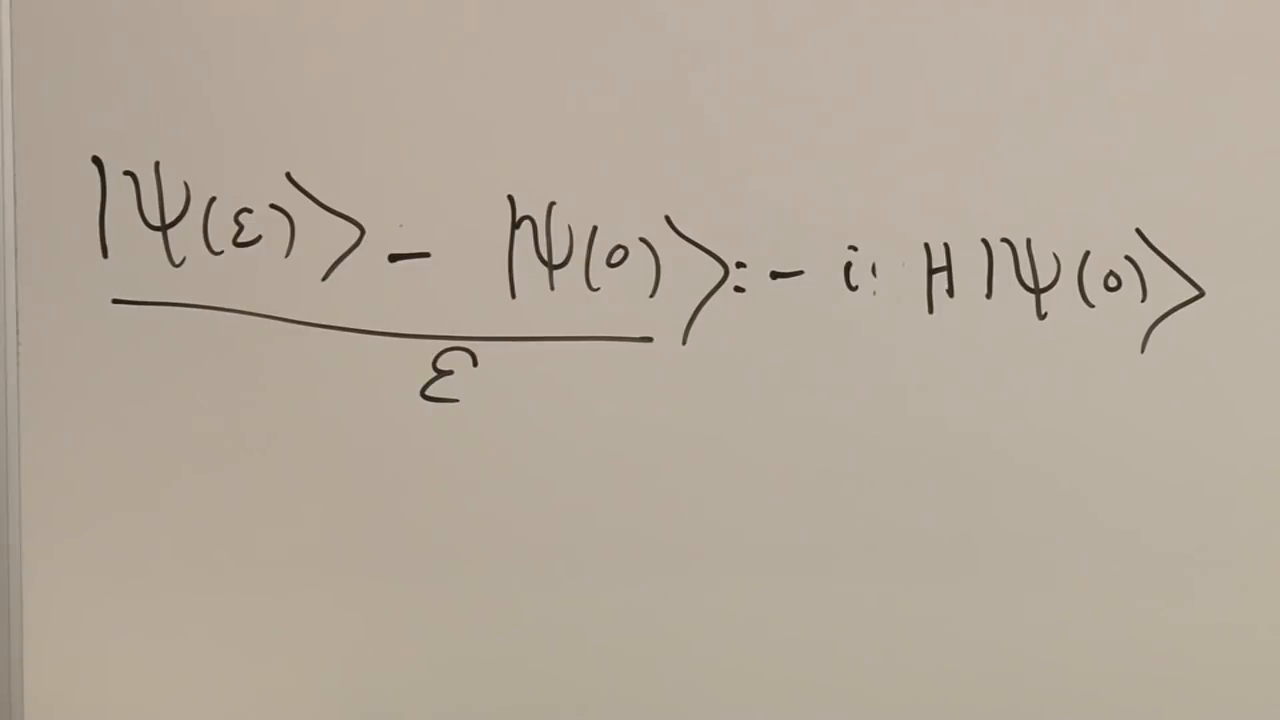
\includegraphics[width=0.86\textwidth]{lecture_05_figure_03.png}\caption{차분 몫으로 쓴 무한소 시간 갱신.}\lectureframe{00:23:33}\end{figure}

\(\epsilon\to0\)의 극한을 취하면 시간 의존 Schr\"odinger 방정식을 얻는다.
\begin{equation}
\frac{d}{dt}\ket{\psi(t)}=-iH\ket{\psi(t)}.
\label{eq:l5-schrodinger}
\end{equation}
상수를 복원하면 이 식은 \(i\hbar\,d\ket{\psi}/dt=H\ket{\psi}\)이다.

Schr\"odinger의 원래 방정식은 운동하는 입자의 파동함수에 관한 것이었다. 위의 연산자 방정식은 한때 일반화된 Schr\"odinger 방정식이라 불렸다. 스핀, 세 상태 계, 스핀 두 개, 또는 임의의 복잡성을 지닌 계에도 똑같이 적용되기 때문이다. 일반화된이라는 수식어는 대체로 생략되었으며, 이제는 이 식을 그저 방정식의 일반형이라고 부른다.

식~\eqref{eq:l5-schrodinger}은 계를 외부와 격리해 두었을 때 상태가 어떻게 결정론적으로 시간발전하는지 나타낸다. 그렇다고 모든 실험 결과가 확정된다는 뜻은 아니다. 양자 상태는 가능한 측정 결과의 확률을 정하며, 이 방정식은 시간에 따라 변하는 진폭을 통해 그 확률을 갱신한다. 측정은 대체로 상태를 변화시키며, 격리된 계의 시간발전을 중단시킨다.

\begin{classroomqa}\audiencequestion{모든 측정은 계를 교란하나요?}\lecturerresponse{일반적으로는 그렇다. 다만 중요한 특별한 경우가 있다. 상태가 이미 그 관측량의 고유상태라면, 이상적인 반복 가능 측정은 상태를 바꾸지 않고 그 값을 확인할 수 있다. 일반적으로 불가능한 것은 서로 양립하지 않는 다른 성질을 교란하지 않으면서 임의의 관측량을 측정하는 일이다.}\end{classroomqa}

\section{에너지와 시간독립 방정식}

\(H\)은 에르미트이므로 고유값은 실수이고, 고유벡터는 완전한 정규직교 기저가 되도록 선택할 수 있다.
\begin{equation}
H\ket{E_i}=E_i\ket{E_i}.
\label{eq:l5-time-independent}
\end{equation}
이것이 Schr\"odinger 방정식의 시간독립형이다. 운동 방정식이 아니라 고유값 문제로서, 계가 어떤 에너지 값을 가질 수 있는지, 그리고 어떤 상태에서 그 값이 정확히 정해지는지를 묻는다.

스펙트럼은 계에 따라 달라진다. 원자에 속박된 운동과 조화 진동자는 셀 수 있는 에너지 준위를 갖는다. 속박되지 않은 입자는 연속 스펙트럼을 가질 수 있다. 에너지를 측정하는 방법은 여러 가지다. 원리적으로는 충분히 정밀한 질량 측정을 통해서도 \(E=mc^2\)를 이용할 수 있지만, 실제로 그런 방법을 쓰는 일은 드물다. 실제 계에는 이미 해밀토니안이 주어져 있다. 물리학자가 해밀토니안을 정하는 것이 아니라 그것을 알아내려 한다. 그 연산자를 알고 나면 고유값과 고유벡터를 구하는 것이 수학적 과제다.

\(cI\)을 \(H\)에 더하면 모든 에너지가 \(c\)만큼 이동한다. 상태 전체에 공통 위상 \(e^{-ict}\)이 곱해지지만, 이는 확률이나 기댓값을 바꾸지 않는다. 여기서 다루는 시간발전에 영향을 주는 것은 에너지의 차이뿐이다.

\section{기댓값의 시간에 따른 변화}

일반적으로 쓰는 \emph{기댓값}은 통계적 평균을 뜻한다. 관측량 \(L\)에 대해
\begin{equation}
\expect{L}(t)=\bra{\psi(t)}L\ket{\psi(t)}.
\end{equation}
이 단계에서는 상태 벡터에만 시간 의존성이 있다. 양변을 미분하고 식~\eqref{eq:l5-schrodinger} 및 그 에르미트 켤레를 사용하면
\begin{equation}
\frac{d}{dt}\ket{\psi}=-iH\ket{\psi},
\qquad
\frac{d}{dt}\bra{\psi}=i\bra{\psi}H,
\end{equation}
다음을 얻는다.
\begin{align}
\frac{d}{dt}\expect{L}
&=i\bra{\psi}HL\ket{\psi}
  -i\bra{\psi}LH\ket{\psi}\\
&=-i\expect{[L,H]}.
\label{eq:l5-expectation-motion}
\end{align}

\begin{figure}[htbp]\centering
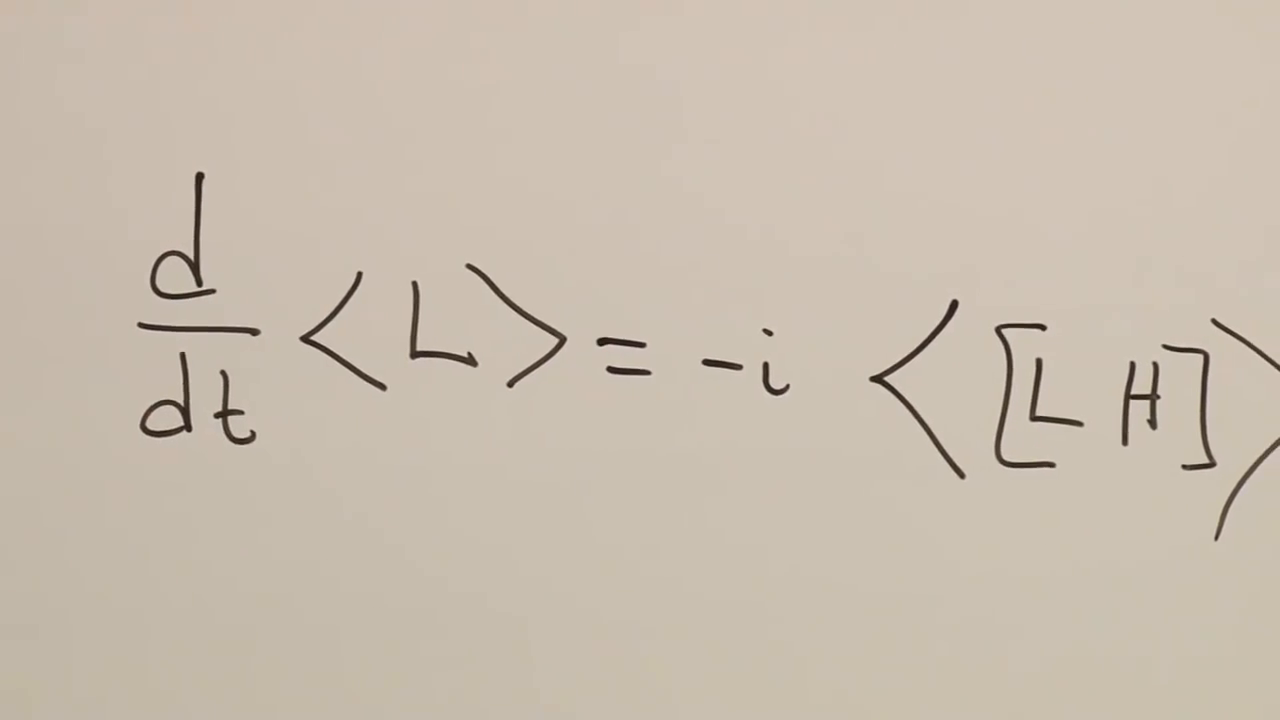
\includegraphics[width=0.86\textwidth]{lecture_05_figure_04.png}\caption{교환자 형태로 쓴 기댓값의 운동 방정식.}\lectureframe{00:35:35}\end{figure}

인자 \(i\)가 있다고 해서 \(\expect{L}\)의 실수성이 위협받는 것은 아니다. 에르미트 연산자 \(L\)와 \(H\)에 대해 교환자는 반에르미트다.
\begin{equation}
[L,H]^\dagger=-[L,H].
\end{equation}
따라서 그 기댓값은 순허수이고, 여기에 \(-i\)를 곱하면 실수인 시간 미분값을 얻는다.

때로는 다음과 같은 약식 표기를 쓴다.
\begin{equation}
\dot L=-i[L,H].
\end{equation}
이 단계에서는 이 표기를 평균에 관한 방정식인 식~\eqref{eq:l5-expectation-motion}의 약기로 읽어야 한다. 연산자 자체가 시간 의존성을 갖는 전체 그림 변환은 뒤에서 다룬다.

\subsection{교환자 대수}

교환자는 반대칭이다.
\begin{equation}
[A,B]=-[B,A].
\end{equation}
또한 미분의 라이프니츠 법칙과 비슷한 곱셈 법칙을 따른다.
\begin{equation}
[AB,C]=A[B,C]+[A,C]B.
\label{eq:l5-product-rule}
\end{equation}
이를 확인하려면 각 인자의 순서를 그대로 유지해야 한다.
\begin{align}
A[B,C]+[A,C]B
&=A(BC-CB)\\
&\quad +(AC-CA)B\\
&=ABC-ACB\\
&\quad +ACB-CAB\\
&=ABC-CAB\\
&=[AB,C].
\end{align}

\begin{figure}[htbp]\centering
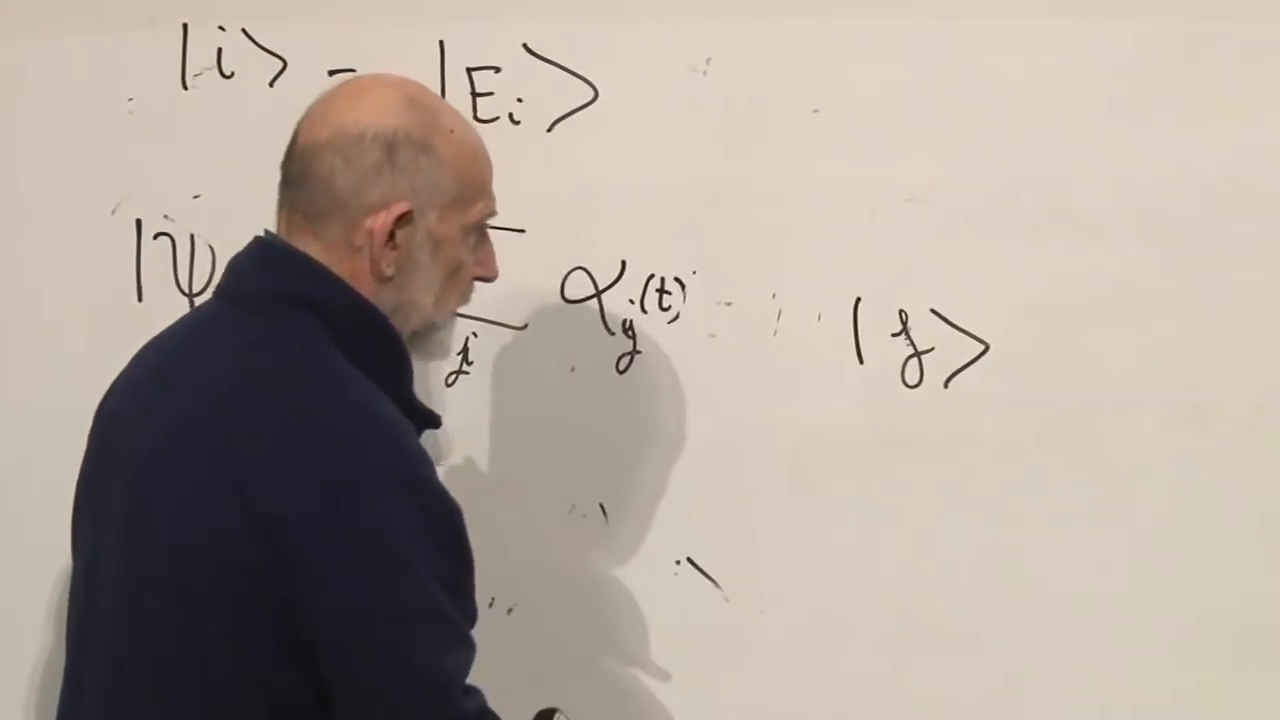
\includegraphics[width=0.86\textwidth]{lecture_05_figure_05.png}\caption{양변을 전개하여 확인한 교환자의 곱셈 법칙.}\lectureframe{00:43:10}\end{figure}

\begin{classroomqa}\audiencequestion{곱셈 법칙의 우변은 좌변을 실수로 두 번 세는 것 아닌가요?}\lecturerresponse{아니다. 전개하면 \(ABC\)와 \(-CAB\)가 원하는 두 항이다. 삽입한 두 항 \(-ACB\)와 \(+ACB\)는 정확히 상쇄된다. 겉보기에는 항이 하나 더 있는 듯하지만, 식을 필요한 두 가지 방식으로 묶기 위해 중간에 넣은 항이다.}\end{classroomqa}

고전적인 푸아송 괄호에도 같은 반대칭성과 곱셈 법칙이 성립한다. 이런 구조적 유사성은 우연이 아니다. 고전적 대응 관계는 다음과 같다.
\begin{equation}
\{A,B\}
\quad\longleftrightarrow\quad
\frac{1}{i\hbar}[A,B]
=-\frac{i}{\hbar}[A,B].
\label{eq:l5-poisson-correspondence}
\end{equation}
\(\hbar=1\)인 단위계에서는 고전 방정식
\begin{equation}
\frac{dL}{dt}=\{L,H\}
\end{equation}
이 식~\eqref{eq:l5-expectation-motion}과 같은 형태를 갖는다. 보통의 거시적 단위계에서 \(\hbar\)는 매우 작고, 적절한 고전적 극한에서는 교환자의 효과가 무시할 수 있을 만큼 작아진다. 이는 양자역학의 생성자 \(H\)가 고전역학의 해밀토니안에 대응함을 확인하는 핵심적인 점검이다.

차원 분석을 해도 인자 \(\hbar\)가 필요하다. 푸아송 괄호는 켤레 좌표와 운동량에 대해 미분하지만, 연산자 교환자는 곱으로 직접 구성된다. 플랑크 상수는 두 차원을 서로 변환해 준다.

\(L=H\)로 두자. 모든 연산자는 자기 자신과 가환하므로
\begin{equation}
\frac{d}{dt}\expect{H}
=-i\expect{[H,H]}=0.
\end{equation}
여기서 다루는 시간독립 해밀토니안에서는 평균 에너지가 보존된다. 에너지 분포 전체에 관한 더 강한 명제도 가능하지만, 여기서는 평균만으로 충분하다.

\begin{classroomqa}\audiencequestion{이 방정식에서 \(L\)는 무엇인가요? 각운동량인가요?}\lecturerresponse{여기서 \(L\)는 일반적인 에르미트 선형 연산자, 즉 임의의 관측량이다. 스핀 성분이나 위치일 수도 있고, \(H\) 자체일 수도 있다. 이 문자는 \emph{선형 연산자}를 뜻하도록 선택했으므로, 별도로 명시되지 않는 한 각운동량으로 해석해서는 안 된다.}\end{classroomqa}

\begin{classroomqa}\audiencequestion{인자 \(i\)가 어떻게 실수인 평균의 미분값을 허수가 아니게 하나요?}\lecturerresponse{에르미트 연산자 두 개의 교환자는 반에르미트이므로 그 기댓값은 허수다. 아래에서 파울리 행렬을 계산하면 이 점이 구체적으로 드러난다. 파울리 행렬의 교환자에는 명시적으로 인자 \(2i\)가 들어 있어 운동 방정식의 \(-i\)와 상쇄된다.}\end{classroomqa}

\section{Schr\"odinger 방정식을 에너지 기저에서 풀기}

에너지 고유값 문제를 이미 풀었다고 하자. 고정된 에너지 기저에서 임의의 상태를 전개하면
\begin{equation}
\ket{\psi(t)}=\sum_j\alpha_j(t)\ket{E_j}.
\label{eq:l5-energy-expansion}
\end{equation}
이 표현에서는 기저 벡터가 변하지 않으며, 모든 시간 의존성은 계수에 들어 있다. 식~\eqref{eq:l5-energy-expansion}을 식~\eqref{eq:l5-schrodinger}에 대입하면
\begin{align}
\sum_j\dot\alpha_j(t)\ket{E_j}
&=-i\sum_j\alpha_j(t)H\ket{E_j}\\
&=-i\sum_j E_j\alpha_j(t)\ket{E_j}.
\end{align}
기저 전개의 유일성에 따라 고정된 \(j\)마다 다음이 성립한다.
\begin{equation}
\dot\alpha_j(t)=-iE_j\alpha_j(t),
\qquad\text{no sum on \(j\)}.
\end{equation}
해는 다음과 같다.
\begin{equation}
\alpha_j(t)=\alpha_j(0)e^{-iE_jt}.
\label{eq:l5-energy-phase}
\end{equation}

\begin{figure}[htbp]\centering
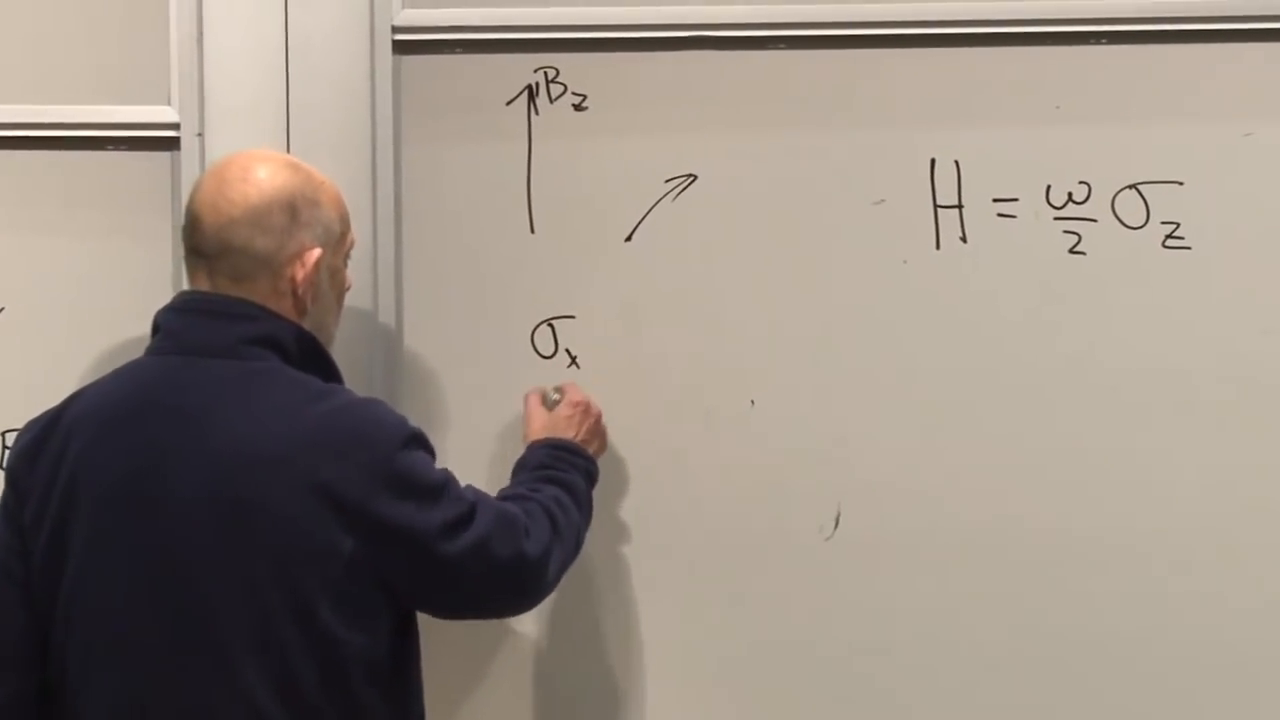
\includegraphics[width=0.86\textwidth]{lecture_05_figure_06.png}\caption{에너지 기저의 각 전개 계수는 독립적으로 지수 위상 방정식을 따른다.}\lectureframe{01:03:25}\end{figure}

따라서 일반해는 다음과 같다.
\begin{equation}
\ket{\psi(t)}
=\sum_j\alpha_j(0)e^{-iE_jt}\ket{E_j}.
\label{eq:l5-general-solution}
\end{equation}
단위를 복원하면 \(E_jt\)는 \(E_jt/\hbar\)로 바뀐다. 모든 계수의 크기는 그대로 유지된다.
\begin{equation}
|\alpha_j(t)|=|\alpha_j(0)|.
\end{equation}
시간발전은 상대 위상을 바꾼다. 에너지 고유상태 하나는 공통 위상 하나만 얻으므로 측정 확률은 시간에 따라 변하지 않는다.

이제 \(L\)의 기댓값을 명시적으로 쓸 수 있다. 에너지 기저에서 행렬 원소를 다음과 같이 정의하자.
\begin{equation}
L_{kj}=\bra{E_k}L\ket{E_j}.
\end{equation}
그러면
\begin{align}
\expect{L}(t)
&=\sum_{k,j}
\alpha_k^*(0)\alpha_j(0)
e^{i(E_k-E_j)t}
L_{kj}.
\label{eq:l5-heisenberg-matrix}
\end{align}

\begin{figure}[htbp]\centering
\includegraphics[width=0.86\textwidth]{lecture_05_figure_07.png}\caption{에너지 기저의 행렬 공식: 각 원소에는 전이 진동수에 따른 위상이 들어 있다.}\lectureframe{01:10:45}\end{figure}

대각항 \(k=j\)은 상수다. 비대각 행렬 원소는 에너지 차이 \(E_k-E_j\)에 따라 진동한다. 여기서 다루는 역사적 설명에 따르면, 하이젠베르크는 현대적인 상태 벡터 유도가 나오기 전에 이런 행렬 구조를 알아보았다. 이후 디랙의 표기법이 그 의미를 명료하게 해 주었다.

\begin{classroomqa}\audiencequestion{계수 \(\alpha_j\)의 크기는 그대로 유지되나요?}\lecturerresponse{그렇다. 각 계수에는 크기가 1인 복소 위상이 곱해진다. 변하는 것은 상대 위상뿐이며, 비대각 행렬 원소를 포함하는 기댓값이 시간에 따라 변할 수 있는 이유가 바로 그 위상이다.}\end{classroomqa}

\begin{classroomqa}\audiencequestion{Schr\"odinger 방정식에는 편미분을 써야 하나요, 전미분을 써야 하나요?}\lecturerresponse{여기서 쓰는 추상 상태 \(\ket{\psi(t)}\)에는 시간만 변수로 나타나 있으므로, 어느 표기법을 써도 내용은 같다. 나중에 \(\psi(x,t)\)와 같은 파동함수는 위치와 시간 모두에 의존하게 되며, 그때는 편미분 표기가 자연스럽다.}\end{classroomqa}

\begin{classroomqa}\audiencequestion{직교성 보존은 단지 경험적 가정인가요?}\lecturerresponse{실험이 이를 뒷받침하지만, 직교성 보존은 유난히 견고한 성질이기도 하다. 유니터리 양자역학을 변형하려는 시도는 양의 정부호성이나 확률 보존, 인과적 국소성, 또는 합성계의 일관된 취급을 무너뜨리는 경향이 있다. 데이비드 핀켈슈타인은 변형 가능한 이론은 소성 유동을 겪고, 견고한 이론은 취성 파괴를 겪는다고 설명했다. 이런 의미에서 양자역학은 취성적이다. 임의로 조금 바꾸더라도 대개 그에 가까운 일관된 이론이 남지 않는다.}\end{classroomqa}

\begin{classroomqa}\audiencequestion{에너지 고유값 \(E_j\)가 실수인 이유는 무엇인가요?}\lecturerresponse{유니터리성은 무한소 생성자 \(H\)가 에르미트임을 뜻하며, 에르미트 연산자의 모든 고유값은 실수다. 따라서 직교성 보존에서 유니터리성으로, 다시 \(H\)의 에르미트성으로 이어지고, 그 결과 에너지 스펙트럼이 실수가 된다.}\end{classroomqa}

\section{자기장 속 스핀}

스핀 하나에는 어떤 해밀토니안을 부여해야 할까? 텅 빈 공간에 고립된 스핀에는 특별히 선호되는 방향이 없으므로, 그 해밀토니안은 항등 연산자에 비례하며 관측 가능한 운동을 일으키지 않는다. 자기장은 상호작용 에너지와 축을 함께 제공한다.

자기장이 \(z\) 방향을 향한다고 하자. 전하를 띤 입자는 스핀을 지니며 자기 모멘트도 갖는다. 익숙한 쌍극자 에너지는 그 모멘트와 자기장의 정렬 정도에 비례한다. 자기장 세기, 자기 모멘트, 부호 규약, 그리고 \(\hbar\)를 하나의 상수 \(\omega\)에 흡수하자.
\begin{equation}
H=\frac{\omega}{2}\sigma_z.
\label{eq:l5-z-hamiltonian}
\end{equation}
파울리 교환자에 \(2\)가 들어 있으므로 인자 \(1/2\)를 쓰면 편리하다.

고전적인 화살표 그림은 신중하게 다뤄야 한다. 양자 스핀은 \(x\), \(y\), \(z\) 성분을 동시에 확정된 값으로 갖지 않으므로, 보통의 화살표 하나로 그 모든 성질을 한꺼번에 나타낼 수는 없다. 유용한 3차원 대상은 기댓값 벡터이지, 두 성분으로 이루어진 상태 벡터 자체가 아니다.

\subsection{파울리 교환자}

행렬 표현을 사용하자.
\begin{equation}
\begin{aligned}
\sigma_x&=
\begin{pmatrix}0&1\\1&0\end{pmatrix},\\[0.4em]
\sigma_y&=
\begin{pmatrix}0&-i\\i&0\end{pmatrix},\\[0.4em]
\sigma_z&=
\begin{pmatrix}1&0\\0&-1\end{pmatrix}.
\end{aligned}
\end{equation}
예를 들면
\begin{align}
[\sigma_z,\sigma_x]
&=
\begin{pmatrix}1&0\\0&-1\end{pmatrix}
\begin{pmatrix}0&1\\1&0\end{pmatrix}
-
\begin{pmatrix}0&1\\1&0\end{pmatrix}
\begin{pmatrix}1&0\\0&-1\end{pmatrix}\\
&=
\begin{pmatrix}0&1\\-1&0\end{pmatrix}
-
\begin{pmatrix}0&-1\\1&0\end{pmatrix}\\
&=2
\begin{pmatrix}0&1\\-1&0\end{pmatrix}
=2i\sigma_y.
\end{align}
순환 관계는 다음과 같다.
\begin{equation}
\begin{aligned}
[\sigma_z,\sigma_x]&=2i\sigma_y,\\
[\sigma_x,\sigma_y]&=2i\sigma_z,\\
[\sigma_y,\sigma_z]&=2i\sigma_x.
\end{aligned}
\label{eq:l5-pauli-commutators}
\end{equation}
두 항목의 순서를 바꾸면 부호도 바뀐다.

\begin{figure}[htbp]\centering
\includegraphics[width=0.86\textwidth]{lecture_05_figure_08.png}\caption{세 파울리 교환자는 파울리 행렬 자체를 순환적으로 생성한다.}\lectureframe{01:33:30}\end{figure}

이 관계에는 각운동량의 고전적 푸아송 괄호와 같은 순환 구조가 있다. 또한 교환의 결과가 원래의 세 연산자 안에서 닫히므로 운동 방정식이 특히 간단해진다.

\begin{classroomqa}\audiencequestion{교환자를 브라-켓 괄호를 써서 계산해야 하나요?}\lecturerresponse{아니다. 연산자 곱은 행렬 곱으로 나타낼 수 있으므로, \(2\times2\) 행렬을 이용하면 바로 계산하기 편하다. 또는 위와 아래 기저 상태에 연산자를 차례로 작용시켜도 같은 결과를 얻는다.}\end{classroomqa}

\subsection{기댓값의 세차}

해밀토니안이 식~\eqref{eq:l5-z-hamiltonian}에 주어져 있을 때 식~\eqref{eq:l5-expectation-motion}을 적용하면 다음과 같다.
\begin{align}
\frac{d}{dt}\expect{\sigma_x}
&=-i\frac{\omega}{2}\expect{[\sigma_x,\sigma_z]}
=-\omega\expect{\sigma_y},\\
\frac{d}{dt}\expect{\sigma_y}
&=-i\frac{\omega}{2}\expect{[\sigma_y,\sigma_z]}
=+\omega\expect{\sigma_x},\\
\frac{d}{dt}\expect{\sigma_z}
&=-i\frac{\omega}{2}\expect{[\sigma_z,\sigma_z]}
=0.
\label{eq:l5-spin-motion}
\end{align}

\begin{figure}[htbp]\centering
\begin{minipage}[c]{0.62\textwidth}\centering
\includegraphics[width=\textwidth]{lecture_05_figure_09.png}\end{minipage}\hfill
\begin{minipage}[c]{0.31\textwidth}\centering
\begin{tikzpicture}[scale=0.78,>=Latex]
  \draw[->,thick] (0,0) -- (0,3.0) node[above] {\(z\parallel\bm B\)};
  \draw[dashed] (0,1.8) ellipse (1.45 and 0.42);
  \draw[->,very thick] (0,0) -- (1.05,1.8)
    node[right] {\(\expect{\bm\sigma}\)};
  \draw[->,thick] (1.38,1.67)
    arc[start angle=-12,end angle=245,x radius=1.45,y radius=0.42];
\end{tikzpicture}\end{minipage}\caption{칠판의 방정식과 그 기하학적 결과: 횡방향 기댓값은 회전하고 자기장과 나란한 성분은 일정하게 유지된다. 화살표는 숨은 고전적 스핀이 아니라 세 기댓값을 나타낸다.}\lectureframe{01:35:28}\end{figure}

처음 두 방정식은 횡방향 평면에서의 원운동을 나타낸다.
\begin{align}
\expect{\sigma_x}(t)
&=\expect{\sigma_x}(0)\cos\omega t
-\expect{\sigma_y}(0)\sin\omega t,\\
\expect{\sigma_y}(t)
&=\expect{\sigma_x}(0)\sin\omega t
+\expect{\sigma_y}(0)\cos\omega t.
\end{align}
한편 \(\expect{\sigma_z}\)은 일정하다. 따라서 기댓값 벡터는 각진동수 \(\omega\)로 자기장 축을 중심으로 세차한다.

이 Schr\"odinger 그림에서 연산자는 고정된 행렬이다. 변하는 것은 상태이며, 따라서 기댓값이 익숙한 자이로스코프 운동을 한다.

\begin{classroomqa}\audiencequestion{2차원 상태 공간에서 어떻게 3차원 세차 그림이 나올 수 있나요?}\lecturerresponse{상태 벡터는 정규화 조건과 전체 위상을 제외하면 두 개의 복소 성분으로 이루어진다. 반면 실공간에 그린 벡터는 \(\bigl(\expect{\sigma_x},\expect{\sigma_y},\expect{\sigma_z}\bigr)\)이다. 이 기댓값들은 상태에 의해 정해지며 블로흐 벡터 그림을 이루지만, 상태 벡터 그 자체는 아니다.}\end{classroomqa}

\section{스핀 하나의 가장 일반적인 해밀토니안}

모든 에르미트 \(2\times2\) 행렬은 다음과 같이 전개할 수 있다.
\begin{equation}
H=aI+b_x\sigma_x+b_y\sigma_y+b_z\sigma_z,
\end{equation}
계수들은 실수다. 항등 연산자 항은 전체 위상만 바꾼다. 나머지 세 계수는 벡터의 성분으로 볼 수 있다. 그 크기를 \(\omega/2\), 방향을 단위 벡터 \(\bm n\)로 나타내면, 자명하지 않은 해밀토니안은 다음과 같다.
\begin{equation}
H=\frac{\omega}{2}\,\bm\sigma\cdot\bm n,
\qquad
\bm\sigma\cdot\bm n
=n_x\sigma_x+n_y\sigma_y+n_z\sigma_z.
\label{eq:l5-general-spin-h}
\end{equation}
\(\bm B=B\bm n\)이라면 \(\bm n\)는 자기장의 방향을 나타내고, \(\omega\)는 자기 결합과 함께 자기장의 크기를 나타낸다. 방향을 기록하는 것은 \(\bm n\)이지 \(\omega\)가 아니다.

운동 방정식은 다음처럼 간결하게 쓸 수 있다.
\begin{equation}
\frac{d}{dt}\expect{\bm\sigma}
=\omega\,\bm n\times\expect{\bm\sigma}.
\end{equation}
\(\bm n\) 방향 성분은 \(H\)와 가환하므로 고정되어 있고, 수직 성분은 \(\bm n\)를 중심으로 세차한다.

\begin{classroomqa}\audiencequestion{왜 해밀토니안이 이 형태여야 하나요?}\lecturerresponse{서로 독립적인 에르미트 \(2\times2\) 행렬은 네 개뿐이다. \(I,\sigma_x,\sigma_y,\sigma_z\)가 그것들이다. 항등 행렬은 스핀 하나의 관측 가능한 운동을 만들지 않으므로, 시간독립적인 스핀 하나의 모든 비자명한 해밀토니안은 파울리 행렬 세 개의 실수 선형결합이다. 자기장은 이 세 계수를 크기와 방향으로 묶어 나타낸다.}\end{classroomqa}

\begin{classroomqa}\audiencequestion{\(\omega\)는 정확히 무엇을 나타내나요?}\lecturerresponse{자기장 크기와 자기 모멘트의 곱에 비례하는 스칼라로, 관례적인 상수들은 여기에 흡수되어 있다. 이 값은 세차율과 에너지 분리를 모두 정한다. 단위 벡터 \(\bm n\)는 자기장의 방향을 나타낸다.}\end{classroomqa}

\subsection{두 에너지 준위}

식~\eqref{eq:l5-general-spin-h}을 행렬로 쓰면 다음과 같다.
\begin{equation}
\bm\sigma\cdot\bm n
=
\begin{pmatrix}
n_z & n_x-in_y\\
n_x+in_y & -n_z
\end{pmatrix}.
\end{equation}
고유값을 \(\lambda_1,\lambda_2\)이라고 하자. 자취는 0이다.
\begin{equation}
\lambda_1+\lambda_2=0.
\end{equation}
단위 벡터 \(n_x^2+n_y^2+n_z^2=1\)의 행렬식은 다음과 같다.
\begin{align}
\lambda_1\lambda_2
&=\det(\bm\sigma\cdot\bm n)\\
&=-n_z^2-(n_x-in_y)(n_x+in_y)\\
&=-(n_x^2+n_y^2+n_z^2)\\
&=-1.
\end{align}
그러므로 두 고유값은 다음과 같다.
\begin{equation}
\lambda_\pm=\pm1.
\end{equation}

\begin{figure}[htbp]\centering
\includegraphics[width=0.86\textwidth]{lecture_05_figure_10.png}\caption{\(\bm\sigma\cdot\bm n\)의 자취와 행렬식으로 고유값이 \(+1\)와 \(-1\)임을 알 수 있다.}\lectureframe{01:59:20}\end{figure}

따라서
\begin{equation}
E_\pm=\pm\frac{\omega}{2},
\qquad
\Delta E=E_+-E_-=\omega.
\label{eq:l5-spin-gap}
\end{equation}
자기장 방향은 에너지 고유벡터를 바꾸지만, 이 두 고유값은 바꾸지 않는다.

\begin{classroomqa}\audiencequestion{광자 방출은 이 에너지 준위와 어떤 관계가 있나요?}\lecturerresponse{복사장을 포함하면 높은 스핀 준위가 낮은 준위로 전이하면서, 여기서 쓰는 \(\hbar=1\) 규약으로 에너지 \(\Delta E=\omega\)인 광자를 방출할 수 있다. 그러면 스핀은 자기장 축을 따라 서로 반대인 두 방향 사이에서 뒤집힌다. 세차 계산에서는 이 약한 복사 결합을 생략했으므로, 스핀은 광자를 방출하기 전에 여러 번 세차할 수 있다.}\end{classroomqa}

\begin{classroomqa}\audiencequestion{왜 자기장은 양자 연산자가 아니라 수로 취급하나요?}\lecturerresponse{자석은 요동과 반동을 무시할 수 있는 무거운 고전적 장치로 잠정적으로 취급한다. 완전한 설명이라면 자석을 더 큰 양자계에 포함해야 한다. 장치가 많은 자유도를 가지고, 관련 변수의 요동이 충분히 작아 전자가 그 변수를 유의미하게 바꾸지 못할 때 실용적인 계와 측정 장치의 분리가 정당화된다.}\end{classroomqa}

\begin{classroomqa}\audiencequestion{매끄러운 세차 방정식은 각각의 개별 시행을 기술하나요?}\lecturerresponse{이 방정식은 기댓값, 즉 동일하게 준비한 여러 시행의 평균을 기술한다. 개별 측정 결과에는 여전히 확률성이 남아 있다. 반복 표본은 이론적 평균에 가까워지는 경향이 있지만, 확률론이 유한한 횟수의 측정에서 정확히 하나의 결과를 보장하는 것은 아니다. 동전을 백만 번 던져도 앞면이 정확히 절반 나와야 하는 것은 아닌 것과 같다.}\end{classroomqa}

\begin{classroomqa}
\audiencequestion{스핀이 횡방향을 향하면 전이 과정에서 광자의 절반을 방출할까요?}
\lecturerresponse{아니다. 횡방향 스핀 상태는 두 에너지 고유상태의 중첩이다. 대칭적인 경우에는 위 에너지 준위와 아래 에너지 준위에 있을 확률이 각각 절반이다. 따라서 에너지가 \(\omega\)인 광자 하나를 온전히 방출하거나, 아무것도 방출하지 않을 수 있다. 평균 방출 에너지는 \(\omega/2\)일 수 있지만, 실제로 방출되는 광자 하나가 에너지 준위 간격의 절반을 갖는 일은 없다.}
\end{classroomqa}

이제 스핀 하나의 비자명한 시간독립 동역학을 모두 살펴보았다. 불확정성을 처음 드러낸 대수 구조가 스핀의 운동도 만들어 낸다. 비가환 파울리 행렬은 해밀토니안을 세차 운동으로 나타내며, 해밀토니안과 가환하는 성분은 보존된다. 다음 단계의 복잡성 증가는 스핀 하나의 해밀토니안을 더 다루는 것이 아니라, 독립된 계들을 합성하고 얽을 수 있는 더 큰 상태 공간으로 나아가는 것이다.
